% --------------------------------------------
% Slight Modification Needed file
% --------------------------------------------

\chapter{Cost Estimation}

\section{Cost Estimation Approach}

The cost estimate was developed using a unit cost–based methodology aligned with the finalized design of the lift station and force main system. Construction costs were derived from a combination of regional data sources, including Mississippi Department of Transportation (MDOT) bid price databases, recent municipal bid tabulations, and published cost references such as RSMeans. Where applicable, costs were adjusted to reflect the project scale, material specifications, and local construction conditions.

Major equipment costs, particularly the selected pump system, were estimated using vendor-based pricing for comparable configurations. Lump-sum values were adopted for components where detailed quantity breakdowns were not necessary at this stage. The estimate incorporates direct construction costs, indirect costs, and engineering-related expenses, along with appropriate allowances for contractor overhead, profit, and contingency, consistent with standard engineering practice and FHWA cost estimating guidance.

\section{Cost Breakdown}

\subsection{Direct Costs}

Direct construction costs represent the primary expenses associated with physically building the lift station and force main system. These costs include materials, labor, and equipment required for installation of structural components, mechanical systems, piping, and sitework. Unit costs were developed using regional bid data from the Mississippi Department of Transportation (MDOT), recent municipal project bid tabulations, and standard construction cost references, with adjustments made to reflect project-specific conditions and scale \cite{MDOT_BidTab_2024, CityMagnolia_BidTab_2024, CityClinton_BidTab_2020, RSMeans_CostData_2025}. Additional market-based pricing for pump station components and wastewater system infrastructure was verified using vendor and municipal cost references to ensure consistency with current construction practices \cite{ExcelFluidGroup_PumpComparison_2024, WaterLevelControls_LiftStationCosts_2024, Wildwood_UtilityCostSchedule_2022}.

\begin{table}[H]
\centering
\caption{Direct Construction Costs}
\label{tab:direct_costs}
\begin{adjustbox}{width=\textwidth}
\begin{tabular}{c l c c c c}
\toprule
\textbf{Item No.} & \textbf{Description} & \textbf{Qty} & \textbf{Unit} & \textbf{Unit Cost (\$)} & \textbf{Line Cost (\$)} \\
\midrule
1  & Sulzer XFP100C VX pumps & 2 & EA & 6,881.22 & 13,762.44 \\
2  & Precast concrete wet well (6-ft dia, 18–20 ft depth) & 1 & LS & 55,000.00 & 55,000.00 \\
3  & Valve vault and discharge assembly & 1 & LS & 22,000.00 & 22,000.00 \\
4  & Discharge piping system, guide rails, fittings & 1 & LS & 14,000.00 & 14,000.00 \\
5  & Check valve and gate valve (4-in) & 1 & LS & 6,500.00 & 6,500.00 \\
6  & Electrical and control system (panel, sensors, wiring) & 1 & LS & 38,000.00 & 38,000.00 \\
7  & Wet well protective coating & 1 & LS & 8,000.00 & 8,000.00 \\
8  & Site excavation, backfill, grading, yard piping & 1 & LS & 22,000.00 & 22,000.00 \\
9  & Access pad / gravel surface / minor site improvements & 1 & LS & 8,000.00 & 8,000.00 \\
10 & Erosion and sediment control & 1 & LS & 4,000.00 & 4,000.00 \\
11 & Quick-connect bypass assembly & 1 & LS & 5,500.00 & 5,500.00 \\
12 & 4-in PVC C900 DR18 force main & 80 & LF & 40.00 & 3,200.00 \\
13 & Trench bedding, backfill, and restoration & 80 & LF & 20.00 & 1,600.00 \\
14 & Force main fittings, tracer wire, markers & 1 & LS & 3,500.00 & 3,500.00 \\
15 & Connection to existing manhole & 1 & LS & 2,500.00 & 2,500.00 \\
16 & Traffic control & 1 & LS & 2,500.00 & 2,500.00 \\
\midrule
\multicolumn{5}{r}{\textbf{Direct Cost Subtotal}} & \textbf{210,062.44} \\
\bottomrule
\end{tabular}
\end{adjustbox}
\end{table}

\subsection{Indirect Costs}

Indirect costs represent supporting construction expenses that are not directly tied to specific quantities of installed work but are necessary for successful project execution. These include site preparation, temporary facilities, utility coordination, and mobilization and demobilization activities required to initiate and complete construction operations. The adopted values were developed based on regional bid tabulations and typical municipal construction practices, with reference to MDOT cost data and recent project bid summaries \cite{MDOT_BidTab_2024, CityMagnolia_BidTab_2024, CertifiedBidTab_Provided_2024}.


\begin{table}[H]
\centering
\caption{Indirect Costs}
\label{tab:indirect_costs}
\begin{tabular}{c l c c c c}
\toprule
17 & Site preparation              & 1 & LS & 6,000.00  & 6,000.00  \\
18 & Temporary facilities          & 1 & LS & 4,000.00  & 4,000.00  \\
19 & Utilities allowance           & 1 & LS & 3,500.00  & 3,500.00  \\
20 & Mobilization / demobilization & 1 & LS & 15,000.00 & 15,000.00 \\
\midrule
\multicolumn{5}{r}{\textbf{Indirect Cost Subtotal}} & \textbf{28,500.00} \\
\bottomrule
\end{tabular}
\end{table}


\subsection{Engineering and Design Costs}

Engineering and design costs include professional services required for planning, investigation, and development of the wastewater conveyance system. These costs consist of surveying for site layout and alignment, geotechnical investigation for subsurface characterization, and design and consulting services for hydraulic, structural, and system design. The values were estimated based on typical ranges observed in municipal infrastructure projects and standard engineering practice, with reference to published cost data and planning-level estimates \cite{CityClinton_ArrowDrive_2025, RSMeans_CostData_2025, FHWA_MajorProjectCostGuidance_2007}.

\begin{table}[H]
\centering
\caption{Engineering and Design Costs}
\label{tab:engineering_costs}
\begin{tabular}{c l c c c c}
\toprule
21 & Surveying                  & 1 & LS & 4,000.00  & 4,000.00  \\
22 & Geotechnical investigation & 1 & LS & 6,000.00  & 6,000.00  \\
23 & Design and consulting fees & 1 & LS & 18,000.00 & 18,000.00 \\
\midrule
\multicolumn{5}{r}{\textbf{Engineering \& Design Subtotal}} & \textbf{28,000.00} \\
\bottomrule
\end{tabular}
\end{table}

\subsection{Overhead, Profit, and Contingency}

Additional project costs include contractor overhead, profit, and contingency allowances, which are applied to the combined direct and indirect construction costs. Contractor overhead accounts for administrative expenses, insurance, and general project management requirements, while profit represents the contractor’s return for undertaking the work. A contingency allowance is included to account for uncertainties associated with material prices, construction conditions, and minor design variations. The selected percentages are consistent with typical ranges recommended in engineering practice and federal cost estimating guidance \cite{FHWA_MajorProjectCostGuidance_2007, RSMeans_CostData_2025}.

\begin{table}[H]
\centering
\caption{Cost Adders: Overhead, Profit, and Contingency}
\label{tab:adders}
\begin{tabular}{l c c c}
\toprule
\textbf{Category} & \textbf{Basis} & \textbf{Rate} & \textbf{Amount (\$)} \\
\midrule
Contractor Overhead & Direct + Indirect & 7\%  & 16,699.37 \\
Contractor Profit   & Direct + Indirect & 7\%  & 16,699.37 \\
Contingency         & Direct + Indirect & 10\% & 23,856.24 \\
\bottomrule
\end{tabular}
\end{table}

\section{Total Project Cost}

The total project cost was determined by combining direct construction costs, indirect costs, engineering and design costs, and applicable contractor adders, including overhead, profit, and contingency. This comprehensive estimate reflects the finalized system design and incorporates all major cost components required for project implementation. The inclusion of contingency and contractor-related costs ensures that the estimate accounts for potential variability in construction conditions and market factors, consistent with standard engineering cost estimation practices \cite{FHWA_MajorProjectCostGuidance_2007}.

\begin{table}[H]
\centering
\caption{Total Project Cost Summary}
\label{tab:total_cost}
\begin{tabular}{l c}
\toprule
\textbf{Category} & \textbf{Amount (\$)} \\
\midrule
Direct Construction Costs & 210,062.44 \\
Indirect Costs            & 28,500.00  \\
Engineering \& Design     & 28,000.00  \\
Contractor Overhead       & 16,699.37  \\
Contractor Profit         & 16,699.37  \\
Contingency               & 23,856.24  \\
\midrule
\textbf{Total Project Cost} & \textbf{323,817.42} \\
\bottomrule
\end{tabular}
\end{table}


\section{Chapter Summary}

The final cost estimate for the proposed wastewater lift station and force main system is based on the finalized hydraulic and layout configuration of the selected design. The proposed system consists of a duplex lift station and an 80-ft-long 4-in PVC force main discharging to the existing municipal sewer system. Using regional bid data, standard cost references, and vendor-based pricing, the estimate was developed to reflect current construction conditions and the major cost components required for implementation \cite{MDOT_BidTab_2024, CityMagnolia_BidTab_2024, CityClinton_BidTab_2020, RSMeans_CostData_2025, FHWA_MajorProjectCostGuidance_2007, Shifat_CostEstimate_2026}.

Direct construction costs constitute the largest share of the budget, totaling \$210{,}062.44. Within this category, the precast concrete wet well, electrical and control system, valve vault and discharge assembly, and excavation-related work represent the dominant cost items. Indirect costs total \$28{,}500.00, while engineering and design costs total \$28{,}000.00. Contractor overhead and profit were each applied at 7\% of the combined direct and indirect construction costs, resulting in \$16{,}699.37 each, and a 10\% contingency allowance was included in the amount of \$23{,}856.24 \cite{Shifat_CostEstimate_2026}.

The distribution of contractor overhead, profit, and contingency is shown in Figure~\ref{fig:adders}. The overall comparison of major project cost components is shown in Figure~\ref{fig:cost_breakdown}. Based on the corrected final estimate, the total project cost is \$323{,}817.42 \cite{Shifat_CostEstimate_2026}. This value represents the full planning-level estimate for the proposed system and provides a practical basis for budgeting and future project development.

\begin{figure}[H]
\centering
\includegraphics[width=0.8\textwidth]{figures/adders.png}
\caption{Distribution of Cost Adders}
\label{fig:adders}
\end{figure}

\begin{figure}[H]
\centering
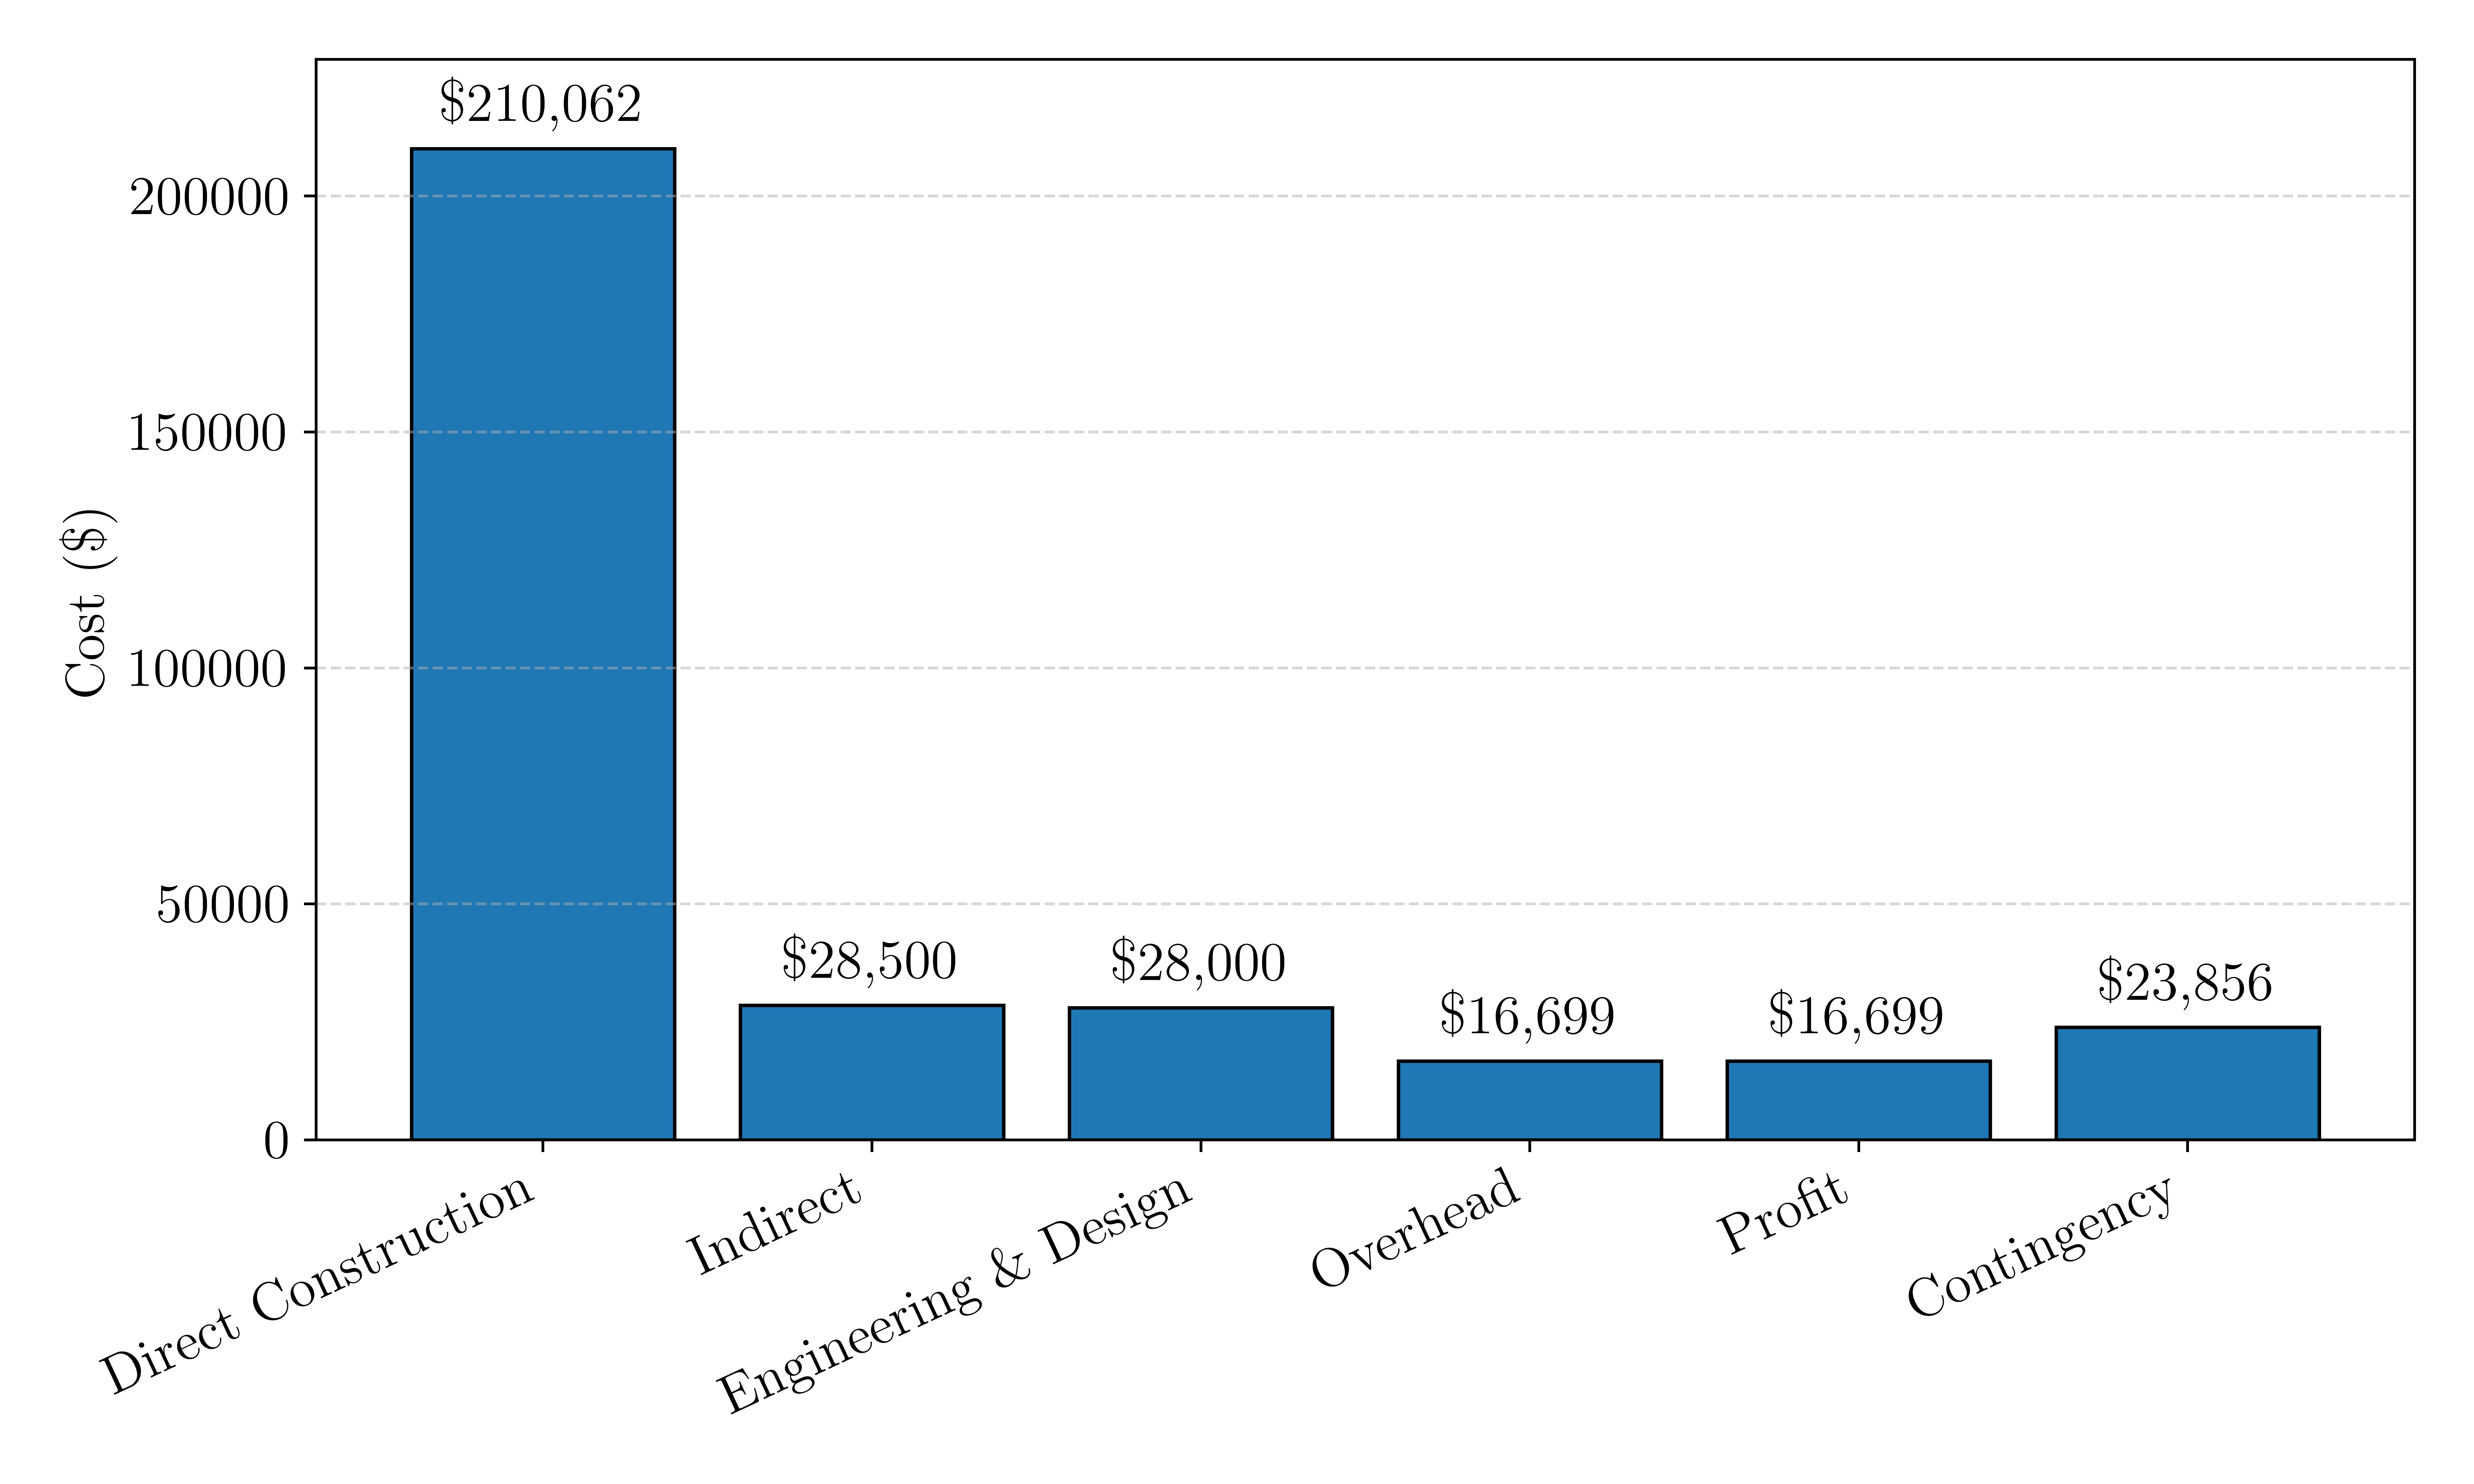
\includegraphics[width=\textwidth]{figures/costing.png}
\caption{Summary of Major Cost Components for the Proposed Lift Station System}
\label{fig:cost_breakdown}
\end{figure}
